\begin{question}
\noindent A school science department has two similar equipment stands used to hold measuring cylinders during experiments. Stand $B$ is an enlargement of Stand $A$.

\begin{center}
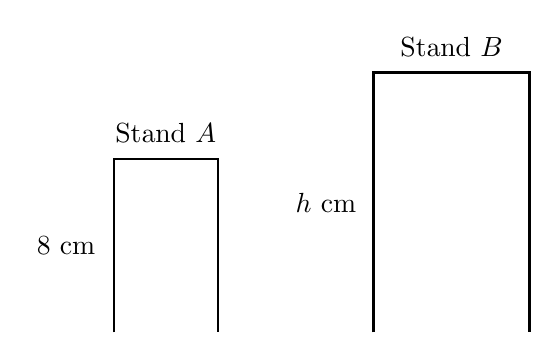
\begin{tikzpicture}[scale=0.55]
    % Stand A (smaller)
    \draw[thick] (0,0) -- (0,4) -- (2.4,4) -- (2.4,0);
    \draw[thick] (0,4) -- (2.4,4);
    \node at (-1.1,2) {$8$ cm};
    \node at (1.2,4.6) {Stand $A$};

    % Stand B (larger, scaled by 1.5)
    \draw[thick] (6,0) -- (6,6) -- (9.6,6) -- (9.6,0);
    \draw[thick] (6,6) -- (9.6,6);
    \node at (4.9,3) {$h$ cm};
    \node at (7.8,6.6) {Stand $B$};
\end{tikzpicture}
\end{center}

\noindent The width of Stand $A$ is $2.4$ cm and the width of Stand $B$ is $3.6$ cm.
The height of Stand $A$ is $8$ cm.

Work out the height, $h$, of Stand $B$.

\vspace{4cm}
\begin{flushright}
\answerequnit{h}{$\text{cm}$}{2}
\end{flushright}
\end{question}
